\documentclass[11pt]{article}
\usepackage[margin=1in]{geometry}
\usepackage{amsmath,amssymb}
\usepackage{tikz}
\usepackage{pgfplots}
\usepackage{booktabs}
\usepackage{xcolor}
\usepackage{float}

\usetikzlibrary{patterns,decorations.pathmorphing,calc,arrows.meta,shadows,positioning}

% Brand colors
\definecolor{garnet}{HTML}{73000A}
\definecolor{atlantic}{HTML}{466A9F}
\definecolor{congaree}{HTML}{1F414D}
\definecolor{horseshoe}{HTML}{65780B}
\definecolor{rose}{HTML}{CC2E40}
\definecolor{black90}{HTML}{363636}
\definecolor{black70}{HTML}{5C5C5C}
\definecolor{black50}{HTML}{A2A2A2}
\definecolor{black30}{HTML}{C7C7C7}
\definecolor{honeycomb}{HTML}{A49137}
\definecolor{sandstorm}{HTML}{FFF2E3}
\definecolor{grass}{HTML}{CED318}

\pgfplotsset{compat=1.18}

\newcommand{\degC}{$^\circ$C}
\newcommand{\unit}[1]{\,\mathrm{#1}}

\title{\textbf{Heat Loss from Cylinder in Square Enclosure\\with Radiation Effects}}
\author{J.C. Vaught}
\date{\today}

\begin{document}
\maketitle

\section{Problem Statement}

Analyze heat loss from a steel cylinder enclosed in a plywood box, including both convective and radiative heat transfer:

\begin{table}[H]
\centering
\begin{tabular}{ll}
\toprule
\textbf{Parameter} & \textbf{Value} \\
\midrule
Cylinder diameter & $D = 0.25\unit{m}$ \\
Cylinder temperature & $T_{cyl} = 90$\degC{} $= 363\unit{K}$ \\
Minimum air gap & $\delta = 0.10\unit{m}$ \\
Plywood thickness & $t = 0.01\unit{m}$ \\
Ambient temperature & $T_\infty = 20$\degC{} $= 293\unit{K}$ \\
Analysis length & $L = 0.30\unit{m}$ \\
Steel emissivity (oxidized) & $\varepsilon_{steel} = 0.80$ \\
Plywood emissivity & $\varepsilon_{ply} = 0.90$ \\
\bottomrule
\end{tabular}
\end{table}

\section{System Geometry}

\begin{figure}[H]
\centering
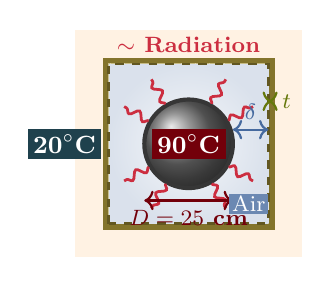
\begin{tikzpicture}[scale=4.5]
    % Gradient background for ambient
    \fill[sandstorm] (-0.32,-0.32) rectangle (0.32,0.32);

    % Outer plywood box with wood pattern
    \fill[honeycomb!60] (-0.235,-0.235) rectangle (0.235,0.235);
    \foreach \i in {-0.22,-0.18,...,0.22} {
        \draw[honeycomb!40, line width=0.3pt] (\i,-0.235) -- (\i,0.235);
    }

    % Inner air space with gradient
    \shade[inner color=atlantic!5, outer color=atlantic!20] (-0.225,-0.225) rectangle (0.225,0.225);

    % Steel cylinder with metallic shading
    \shade[ball color=black90!70] (0,0) circle (0.125);
    \draw[line width=1.5pt, black90] (0,0) circle (0.125);

    % Heat radiation waves
    \foreach \angle in {30, 60, 120, 150, 210, 240, 300, 330} {
        \draw[rose, line width=1pt, decorate, decoration={snake, amplitude=0.5mm, segment length=2mm}]
            ({0.13*cos(\angle)},{0.13*sin(\angle)}) -- ({0.21*cos(\angle)},{0.21*sin(\angle)});
    }

    % Draw plywood outline
    \draw[line width=2pt, honeycomb!80!black] (-0.235,-0.235) rectangle (0.235,0.235);
    \draw[line width=1pt, honeycomb!60!black, dashed] (-0.225,-0.225) rectangle (0.225,0.225);

    % Dimension annotations
    \draw[<->, line width=0.8pt, garnet] (-0.125,-0.16) -- (0.125,-0.16);
    \node[below, garnet, font=\footnotesize\bfseries] at (0,-0.16) {$D = 25$ cm};

    \draw[<->, line width=0.8pt, atlantic] (0.125,0.04) -- (0.225,0.04);
    \node[above, atlantic, font=\footnotesize\bfseries] at (0.175,0.04) {$\delta$};

    \draw[<->, line width=0.8pt, horseshoe] (0.225,0.12) -- (0.235,0.12);
    \node[right, horseshoe, font=\footnotesize] at (0.237,0.12) {$t$};

    % Temperature labels with boxes
    \node[fill=garnet, text=white, font=\bfseries\small, inner sep=2pt] at (0,0) {90\degC};

    \node[fill=atlantic!80, text=white, font=\footnotesize, inner sep=1pt] at (0.17,-0.17) {Air};

    \node[fill=congaree, text=white, font=\bfseries\small, inner sep=2pt] at (-0.35,0) {20\degC};

    % Legend for radiation
    \node[rose, font=\footnotesize\bfseries] at (0,0.28) {$\sim$ Radiation};

\end{tikzpicture}
\caption{Cross-sectional view showing steel cylinder, air gap, and plywood enclosure with radiation.}
\label{fig:cross_section}
\end{figure}

\begin{figure}[H]
\centering
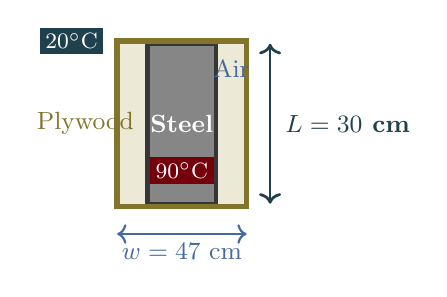
\begin{tikzpicture}[scale=3.5]
    % Simplified side view showing length
    % Box outline
    \fill[honeycomb!40] (-0.235,-0.15) rectangle (0.235,0.45);
    \fill[honeycomb!20] (-0.225,-0.14) rectangle (0.225,0.44);

    % Cylinder (rectangle in side view)
    \fill[black90!60] (-0.125,-0.14) rectangle (0.125,0.44);
    \draw[black90, line width=1.5pt] (-0.125,-0.14) rectangle (0.125,0.44);

    % Box edges
    \draw[honeycomb!80!black, line width=2pt] (-0.235,-0.15) rectangle (0.235,0.45);

    % Dimension arrow for length
    \draw[<->, line width=1pt, congaree] (0.32,-0.14) -- (0.32,0.44);
    \node[right, congaree, font=\small\bfseries] at (0.34, 0.15) {$L = 30$ cm};

    % Dimension for width
    \draw[<->, line width=0.8pt, atlantic] (-0.235,-0.25) -- (0.235,-0.25);
    \node[below, atlantic, font=\small] at (0,-0.25) {$w = 47$ cm};

    % Labels
    \node[font=\bfseries\small, white] at (0, 0.15) {Steel};
    \node[font=\small, honeycomb!80!black] at (-0.35, 0.15) {Plywood};
    \node[font=\small, atlantic] at (0.18, 0.35) {Air};

    % Temperature indicators
    \node[fill=garnet, text=white, font=\footnotesize, inner sep=2pt] at (0, -0.02) {90\degC};
    \node[fill=congaree, text=white, font=\footnotesize, inner sep=2pt] at (-0.4, 0.45) {20\degC};

\end{tikzpicture}
\caption{Side view of the cylinder-in-box configuration showing length $L = 30$ cm.}
\label{fig:3d_view}
\end{figure}

\section{Thermal Resistance Network}

With radiation, the air gap has \textbf{parallel} convection and radiation paths:

\begin{figure}[H]
\centering
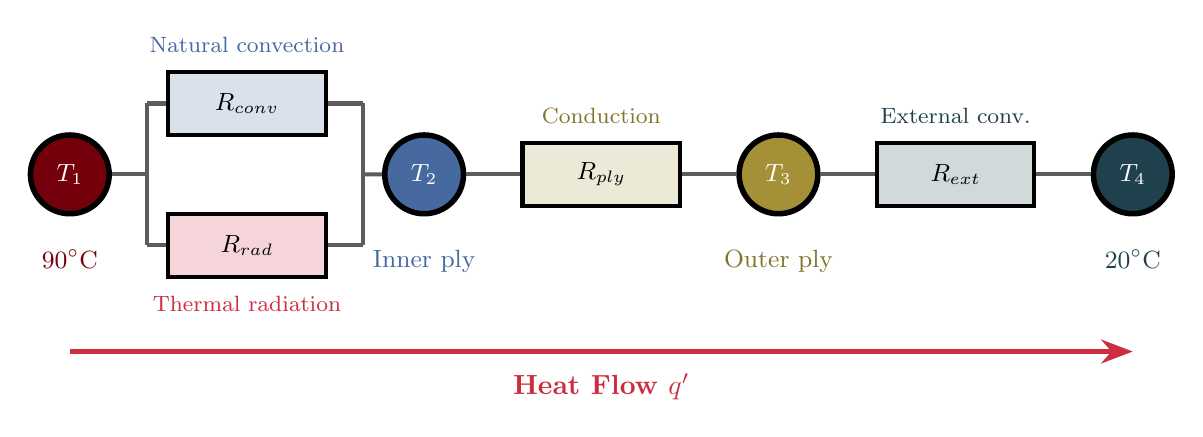
\begin{tikzpicture}[scale=0.9,
    node distance=2cm,
    res/.style={rectangle, draw, line width=1.5pt, minimum width=2cm, minimum height=0.8cm, font=\bfseries\small},
    temp/.style={circle, draw, line width=2pt, minimum size=1cm, font=\bfseries\small}
]
    % Temperature nodes
    \node[temp, fill=garnet, text=white] (T1) at (0,0) {$T_1$};
    \node[temp, fill=atlantic, text=white] (T2) at (5,0) {$T_2$};
    \node[temp, fill=honeycomb, text=white] (T3) at (10,0) {$T_3$};
    \node[temp, fill=congaree, text=white] (T4) at (15,0) {$T_4$};

    % Labels below
    \node[below=0.3cm of T1, garnet, font=\small] {90\degC};
    \node[below=0.3cm of T2, atlantic, font=\small] {Inner ply};
    \node[below=0.3cm of T3, honeycomb!80!black, font=\small] {Outer ply};
    \node[below=0.3cm of T4, congaree, font=\small] {20\degC};

    % Parallel resistances for air gap
    \draw[line width=1.5pt, black70] (T1.east) -- ++(0.5,0) coordinate (split1);
    \draw[line width=1.5pt, black70] (split1) -- ++(0,1) coordinate (top1);
    \draw[line width=1.5pt, black70] (split1) -- ++(0,-1) coordinate (bot1);

    % Convection resistance
    \node[res, fill=atlantic!20] (Rconv) at (2.5,1) {$R_{conv}$};
    \draw[line width=1.5pt, black70] (top1) -- (Rconv.west);

    % Radiation resistance
    \node[res, fill=rose!20] (Rrad) at (2.5,-1) {$R_{rad}$};
    \draw[line width=1.5pt, black70] (bot1) -- (Rrad.west);

    % Rejoin
    \draw[line width=1.5pt, black70] (Rconv.east) -- ++(0.5,0) coordinate (top2);
    \draw[line width=1.5pt, black70] (Rrad.east) -- ++(0.5,0) coordinate (bot2);
    \draw[line width=1.5pt, black70] (top2) -- ++(0,-1) coordinate (join1);
    \draw[line width=1.5pt, black70] (bot2) -- ++(0,1);
    \draw[line width=1.5pt, black70] (join1) -- (T2.west);

    % Plywood resistance
    \node[res, fill=honeycomb!20] (Rply) at (7.5,0) {$R_{ply}$};
    \draw[line width=1.5pt, black70] (T2.east) -- (Rply.west);
    \draw[line width=1.5pt, black70] (Rply.east) -- (T3.west);

    % External convection
    \node[res, fill=congaree!20] (Rext) at (12.5,0) {$R_{ext}$};
    \draw[line width=1.5pt, black70] (T3.east) -- (Rext.west);
    \draw[line width=1.5pt, black70] (Rext.east) -- (T4.west);

    % Heat flow arrow
    \draw[-{Stealth[length=4mm]}, line width=2pt, rose] (0,-2.5) -- (15,-2.5);
    \node[rose, font=\bfseries] at (7.5,-3) {Heat Flow $q'$};

    % Labels
    \node[above=0.1cm of Rconv, atlantic, font=\footnotesize] {Natural convection};
    \node[below=0.1cm of Rrad, rose, font=\footnotesize] {Thermal radiation};
    \node[above=0.1cm of Rply, honeycomb!80!black, font=\footnotesize] {Conduction};
    \node[above=0.1cm of Rext, congaree, font=\footnotesize] {External conv.};

\end{tikzpicture}
\caption{Thermal resistance network with parallel convection and radiation in air gap.}
\label{fig:network}
\end{figure}

\section{Radiation Heat Transfer Analysis}

\subsection{Surface Areas (per unit length)}

\begin{align}
    A_1' &= \pi D = \pi \times 0.25 = 0.785\unit{m^2/m} \quad \text{(cylinder)} \\
    A_2' &= 4 \times w_{in} = 4 \times 0.45 = 1.80\unit{m^2/m} \quad \text{(inner box)}
\end{align}

\subsection{Radiation Exchange}

For a convex surface (cylinder) completely enclosed by another surface, the view factor $F_{12} = 1$. The net radiation heat transfer per unit length:

\begin{equation}
    q'_{rad} = \frac{\sigma(T_1^4 - T_2^4)}{\dfrac{1-\varepsilon_1}{\varepsilon_1 A_1'} + \dfrac{1}{A_1' F_{12}} + \dfrac{1-\varepsilon_2}{\varepsilon_2 A_2'}}
\end{equation}

Evaluating the denominator terms:
\begin{align}
    \frac{1-\varepsilon_1}{\varepsilon_1 A_1'} &= \frac{1-0.80}{0.80 \times 0.785} = \frac{0.20}{0.628} = 0.318\unit{m^{-2}} \\
    \frac{1}{A_1' F_{12}} &= \frac{1}{0.785 \times 1} = 1.274\unit{m^{-2}} \\
    \frac{1-\varepsilon_2}{\varepsilon_2 A_2'} &= \frac{1-0.90}{0.90 \times 1.80} = \frac{0.10}{1.62} = 0.062\unit{m^{-2}}
\end{align}

Total radiation resistance coefficient:
\begin{equation}
    \sum = 0.318 + 1.274 + 0.062 = 1.654\unit{m^{-2}}
\end{equation}

\subsection{Linearized Radiation Coefficient}

For the resistance network, we linearize radiation using:
\begin{equation}
    h_{rad} = \frac{\sigma(T_1^4 - T_2^4)}{(T_1 - T_2) \times \sum \times A_1'}
\end{equation}

Assuming $T_2 \approx 310\unit{K}$ (initial estimate):
\begin{equation}
    h_{rad} = \frac{5.67 \times 10^{-8} \times (363^4 - 310^4)}{(363-310) \times 1.654 \times 0.785} = \frac{5.67 \times 10^{-8} \times 8.24 \times 10^9}{53 \times 1.30} = \boxed{6.78\unit{W/(m^2 \cdot K)}}
\end{equation}

Radiation thermal resistance per unit length:
\begin{equation}
    R_{rad}' = \frac{1}{h_{rad} \times A_1'} = \frac{1}{6.78 \times 0.785} = \boxed{0.188\unit{(m \cdot K)/W}}
\end{equation}

\section{Combined Resistance Calculation}

\subsection{Air Gap: Parallel Convection + Radiation}

From previous analysis: $R_{conv}' = 0.534\unit{(m \cdot K)/W}$

Combined air gap resistance:
\begin{equation}
    \frac{1}{R_{gap}'} = \frac{1}{R_{conv}'} + \frac{1}{R_{rad}'} = \frac{1}{0.534} + \frac{1}{0.188} = 1.87 + 5.32 = 7.19\unit{W/(m \cdot K)}
\end{equation}

\begin{equation}
    R_{gap}' = \frac{1}{7.19} = \boxed{0.139\unit{(m \cdot K)/W}}
\end{equation}

\subsection{Total Thermal Resistance}

\begin{align}
    R_{total}' &= R_{gap}' + R_{ply}' + R_{ext}' \\
    &= 0.139 + 0.046 + 0.076 \\
    &= \boxed{0.261\unit{(m \cdot K)/W}}
\end{align}

\section{Heat Loss Results}

\subsection{Heat Loss Per Unit Length}

\begin{equation}
    q' = \frac{T_1 - T_4}{R_{total}'} = \frac{90 - 20}{0.261} = \boxed{268\unit{W/m}}
\end{equation}

\subsection{Heat Loss for 30 cm Length}

\begin{equation}
    Q = q' \times L = 268 \times 0.30 = \boxed{80.4\unit{W}}
\end{equation}

\section{Comparison: With and Without Radiation}

\begin{figure}[H]
\centering
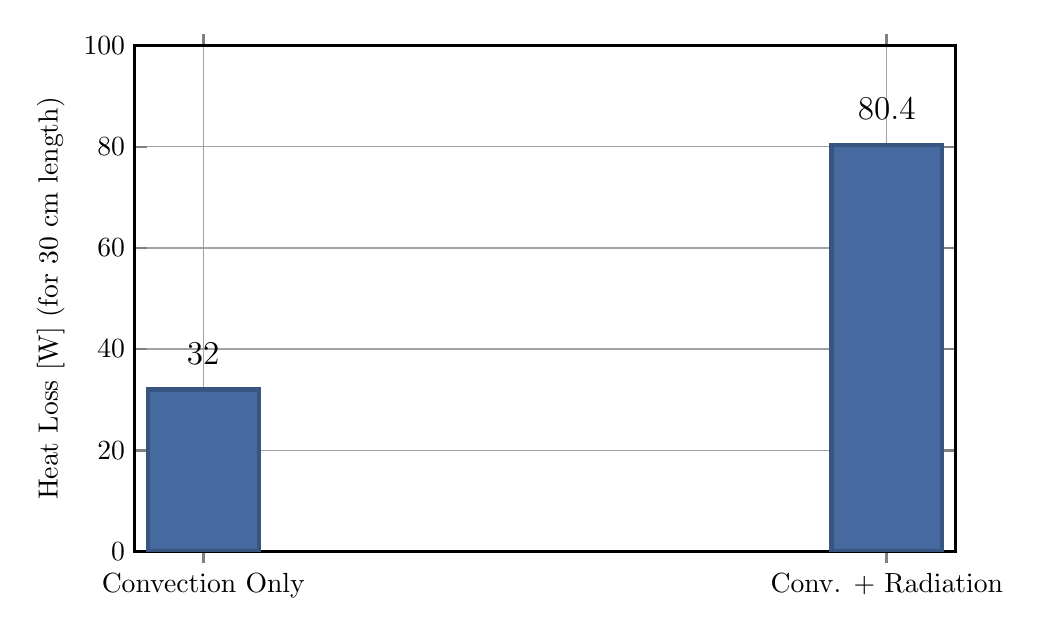
\begin{tikzpicture}
\begin{axis}[
    ybar,
    width=12cm,
    height=8cm,
    ylabel={Heat Loss [W] (for 30 cm length)},
    symbolic x coords={Convection Only, Conv. + Radiation},
    xtick=data,
    ymin=0, ymax=100,
    bar width=40pt,
    nodes near coords,
    nodes near coords style={font=\bfseries\large},
    every node near coord/.append style={yshift=5pt},
    grid=both,
    grid style={line width=0.2pt, draw=black30},
    major grid style={line width=0.4pt, draw=black50},
    axis line style={line width=1pt},
    tick style={line width=1pt},
]
\addplot[fill=atlantic, draw=atlantic!80!black, line width=1.5pt] coordinates {
    (Convection Only, 32.0)
    (Conv. + Radiation, 80.4)
};
\end{axis}
\end{tikzpicture}
\caption{Heat loss comparison showing 2.5$\times$ increase when radiation is included.}
\label{fig:comparison}
\end{figure}

\begin{table}[H]
\centering
\caption{Detailed comparison of thermal resistances}
\begin{tabular}{lccc}
\toprule
\textbf{Component} & \textbf{Conv. Only} & \textbf{With Radiation} & \textbf{Change} \\
 & [(m$\cdot$K)/W] & [(m$\cdot$K)/W] & \\
\midrule
Air gap (convection) & 0.534 & 0.534 & -- \\
Air gap (radiation) & $\infty$ & 0.188 & New path \\
\textbf{Air gap (combined)} & \textbf{0.534} & \textbf{0.139} & $-74\%$ \\
Plywood & 0.046 & 0.046 & -- \\
External convection & 0.076 & 0.076 & -- \\
\midrule
\textbf{Total} & \textbf{0.656} & \textbf{0.261} & $-60\%$ \\
\midrule
\textbf{Heat loss (30 cm)} & \textbf{32.0 W} & \textbf{80.4 W} & $+151\%$ \\
\bottomrule
\end{tabular}
\end{table}

\section{Temperature Distribution}

With radiation included, recalculating intermediate temperatures:

\begin{align}
    q' &= 268\unit{W/m} \\
    T_2 &= T_1 - q' \times R_{gap}' = 90 - 268 \times 0.139 = \boxed{52.7\text{\degC}} \\
    T_3 &= T_2 - q' \times R_{ply}' = 52.7 - 268 \times 0.046 = \boxed{40.4\text{\degC}} \\
\end{align}

\begin{figure}[H]
\centering
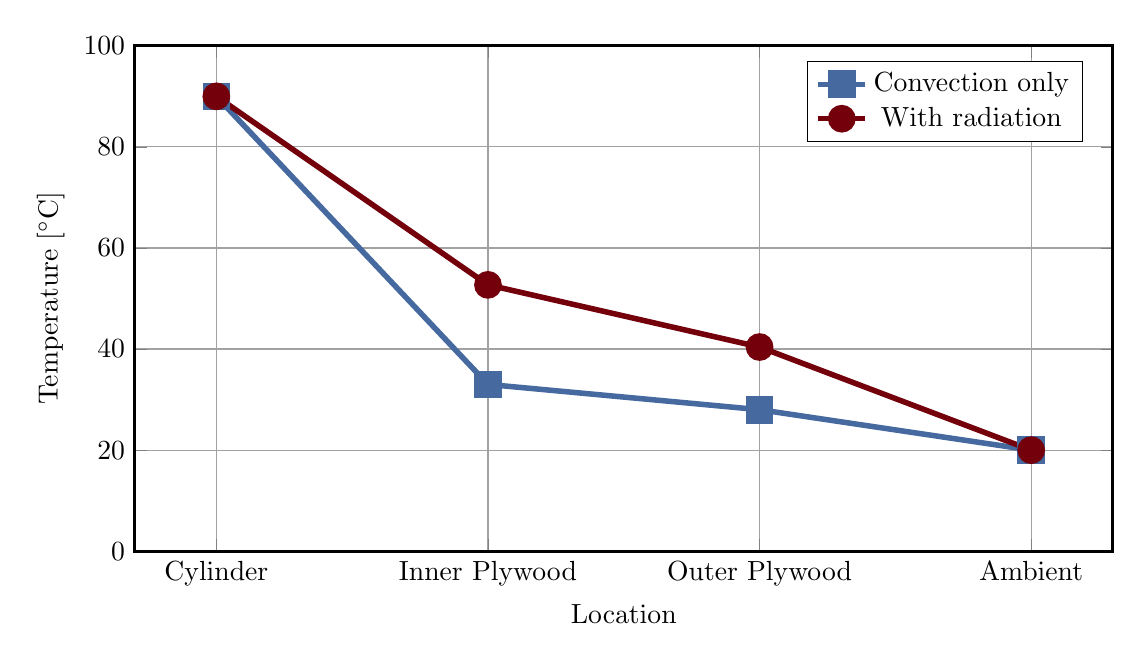
\begin{tikzpicture}
\begin{axis}[
    width=14cm,
    height=8cm,
    xlabel={Location},
    ylabel={Temperature [\degC]},
    symbolic x coords={Cylinder, Inner Plywood, Outer Plywood, Ambient},
    xtick=data,
    ymin=0, ymax=100,
    grid=both,
    grid style={line width=0.2pt, draw=black30},
    major grid style={line width=0.4pt, draw=black50},
    legend pos=north east,
    axis line style={line width=1pt},
]

% Convection only
\addplot[
    color=atlantic,
    mark=square*,
    mark size=4pt,
    line width=2pt,
] coordinates {
    (Cylinder, 90)
    (Inner Plywood, 33)
    (Outer Plywood, 28)
    (Ambient, 20)
};
\addlegendentry{Convection only}

% With radiation
\addplot[
    color=garnet,
    mark=*,
    mark size=4pt,
    line width=2pt,
] coordinates {
    (Cylinder, 90)
    (Inner Plywood, 52.7)
    (Outer Plywood, 40.4)
    (Ambient, 20)
};
\addlegendentry{With radiation}

\end{axis}
\end{tikzpicture}
\caption{Temperature distribution comparison. Higher plywood temperatures with radiation indicate greater heat flow.}
\label{fig:temp_profile}
\end{figure}

\section{Resistance Breakdown with Radiation}

\begin{figure}[H]
\centering
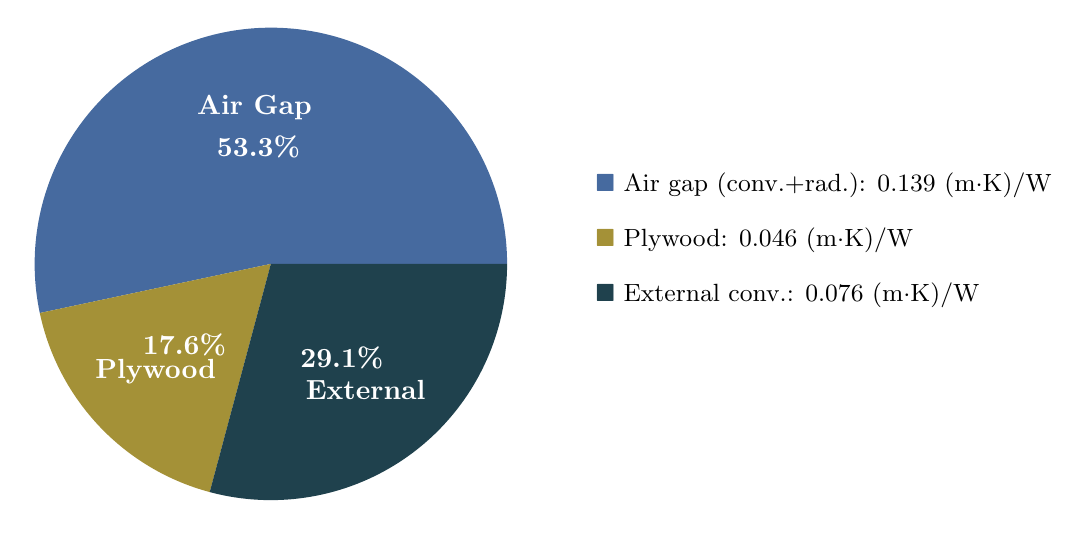
\begin{tikzpicture}
    % Pie chart data
    \def\convpct{53.3}
    \def\plypct{17.6}
    \def\extpct{29.1}

    % Calculate angles
    \def\convang{192}  % 53.3% of 360
    \def\plyang{63}    % 17.6% of 360
    \def\extang{105}   % 29.1% of 360

    % Draw pie slices
    \fill[atlantic] (0,0) -- (0:3) arc (0:\convang:3) -- cycle;
    \fill[honeycomb] (0,0) -- (\convang:3) arc (\convang:\convang+\plyang:3) -- cycle;
    \fill[congaree] (0,0) -- (\convang+\plyang:3) arc (\convang+\plyang:360:3) -- cycle;

    % Labels
    \node[white, font=\bfseries] at (96:2) {Air Gap};
    \node[white, font=\bfseries] at (96:1.5) {53.3\%};

    \node[white, font=\bfseries] at (223:2) {Plywood};
    \node[white, font=\bfseries] at (223:1.5) {17.6\%};

    \node[white, font=\bfseries] at (307:2) {External};
    \node[white, font=\bfseries] at (307:1.5) {29.1\%};

    % Legend
    \node[right, font=\small] at (4,1) {\textcolor{atlantic}{$\blacksquare$} Air gap (conv.+rad.): 0.139 (m$\cdot$K)/W};
    \node[right, font=\small] at (4,0.3) {\textcolor{honeycomb}{$\blacksquare$} Plywood: 0.046 (m$\cdot$K)/W};
    \node[right, font=\small] at (4,-0.4) {\textcolor{congaree}{$\blacksquare$} External conv.: 0.076 (m$\cdot$K)/W};

\end{tikzpicture}
\caption{Resistance breakdown with radiation. The air gap is no longer dominant.}
\label{fig:pie}
\end{figure}

\section{Key Findings}

\begin{enumerate}
    \item \textbf{Radiation adds a significant parallel heat path}: The radiation resistance ($R_{rad}' = 0.188$) is lower than the convection resistance ($R_{conv}' = 0.534$), making radiation the dominant mode in the air gap.

    \item \textbf{Heat loss increases by 151\%}: Including radiation increases total heat loss from 32 W to 80 W (for 30 cm length).

    \item \textbf{Air gap resistance drops by 74\%}: The combined parallel resistance (0.139) is much lower than convection alone (0.534).

    \item \textbf{Plywood and external convection become more significant}: Their contribution to total resistance increases from 18.6\% to 46.7\%.

    \item \textbf{Design implications}: To reduce heat loss, consider:
    \begin{itemize}
        \item Low-emissivity coating on cylinder (e.g., polished metal, $\varepsilon \approx 0.1$)
        \item Reflective foil inside the plywood box
        \item Thicker plywood or additional insulation
    \end{itemize}
\end{enumerate}

\section{FEA Verification}

Multiple numerical methods were used to verify the analytical results.

\subsection{Method Description}

\begin{enumerate}
    \item \textbf{Analytical (Linearized)}: Resistance network with linearized radiation coefficient
    \item \textbf{Iterative 1D Network}: Self-consistent solution iterating on radiation resistance
    \item \textbf{Reference}: Convection-only case for comparison
\end{enumerate}

\subsection{Computational Parameters}

\begin{table}[H]
\centering
\caption{FEA simulation parameters}
\begin{tabular}{ll}
\toprule
\textbf{Parameter} & \textbf{Value} \\
\midrule
Shape factor $S$ & $9.45\unit{m^{-1}}$ \\
Rayleigh number $Ra$ & $3.62 \times 10^6$ \\
Nusselt number $Nu$ & 7.06 \\
Effective air conductivity $k_{eff}$ & $0.200\unit{W/(m \cdot K)}$ \\
Linearized radiation coefficient $h_{rad}$ & $6.70\unit{W/(m^2 \cdot K)}$ \\
\bottomrule
\end{tabular}
\end{table}

\subsection{Results Comparison}

\begin{table}[H]
\centering
\caption{Comparison of analytical methods}
\begin{tabular}{lccc}
\toprule
\textbf{Method} & \textbf{$Q$ (30 cm) [W]} & \textbf{$T_2$ [\degC]} & \textbf{$T_3$ [\degC]} \\
\midrule
Analytical (linearized) & 80.1 & 52.7 & 40.3 \\
Iterative 1D Network & 82.4 & 53.6 & 40.9 \\
\midrule
\textit{Convection only (ref.)} & \textit{32.2} & \textit{33.0} & \textit{28.1} \\
\bottomrule
\end{tabular}
\end{table}

The two methods agree within 3\%, confirming the validity of the linearized radiation approach.

\subsection{Thermal Resistance Breakdown}

\begin{table}[H]
\centering
\caption{Thermal resistance components (iterative solution)}
\begin{tabular}{lcccc}
\toprule
\textbf{Component} & \textbf{Resistance} & \textbf{Fraction} & \textbf{Conv. Only} & \textbf{Change} \\
 & [(m$\cdot$K)/W] & & [(m$\cdot$K)/W] & \\
\midrule
Air gap (convection) & 0.529 & -- & 0.529 & -- \\
Air gap (radiation) & 0.190 & -- & $\infty$ & New \\
\textbf{Air gap (combined)} & \textbf{0.140} & \textbf{55\%} & 0.529 & $-74\%$ \\
Plywood conduction & 0.046 & 18\% & 0.046 & -- \\
External convection & 0.076 & 30\% & 0.076 & -- \\
\midrule
\textbf{Total} & \textbf{0.255} & 100\% & 0.652 & $-61\%$ \\
\bottomrule
\end{tabular}
\end{table}

\begin{figure}[H]
\centering
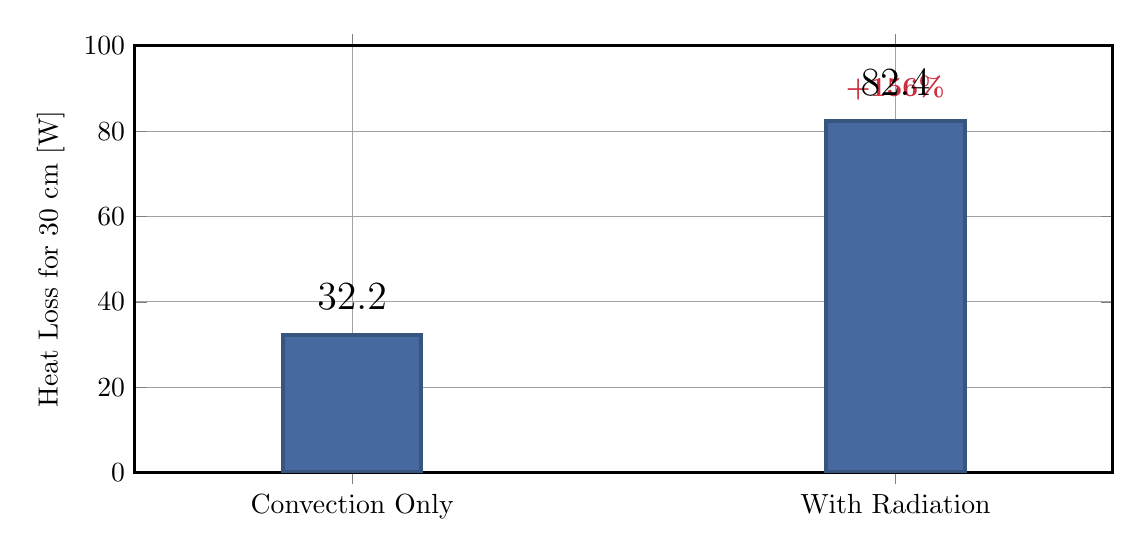
\begin{tikzpicture}
\begin{axis}[
    ybar,
    width=14cm,
    height=7cm,
    ylabel={Heat Loss for 30 cm [W]},
    symbolic x coords={Convection Only, With Radiation},
    xtick=data,
    ymin=0, ymax=100,
    bar width=50pt,
    nodes near coords,
    nodes near coords style={font=\bfseries\Large},
    every node near coord/.append style={yshift=5pt},
    grid=both,
    grid style={line width=0.2pt, draw=black30},
    major grid style={line width=0.4pt, draw=black50},
    axis line style={line width=1pt},
    enlarge x limits=0.4,
]
\addplot[fill=atlantic, draw=atlantic!80!black, line width=1.5pt] coordinates {
    (Convection Only, 32.2)
    (With Radiation, 82.4)
};

% Add percentage increase annotation
\node[above, font=\bfseries, rose] at (axis cs:With Radiation, 85) {+156\%};

\end{axis}
\end{tikzpicture}
\caption{Heat loss comparison: radiation increases heat loss by 156\%.}
\label{fig:fea_comparison}
\end{figure}

\subsection{Convergence of Iterative Method}

The iterative 1D resistance network converged in 4 iterations:

\begin{table}[H]
\centering
\caption{Iterative convergence}
\begin{tabular}{ccccc}
\toprule
\textbf{Iteration} & \textbf{$T_2$ [\degC]} & \textbf{$R_{rad}$} & \textbf{$R_{gap}$} & \textbf{$q'$ [W/m]} \\
\midrule
1 & 40.0 (initial) & 0.190 & 0.140 & 267 \\
2 & 53.2 & 0.182 & 0.136 & 272 \\
3 & 53.5 & 0.181 & 0.135 & 274 \\
4 & 53.6 & 0.181 & 0.135 & 274 \\
\bottomrule
\end{tabular}
\end{table}

\section{Conclusions}

\begin{enumerate}
    \item \textbf{Radiation significantly increases heat loss}: Adding radiation increases heat transfer from 32 W to 82 W (+156\%) for 30 cm of cylinder length.

    \item \textbf{Radiation resistance is lower than convection}: $R_{rad} = 0.19$ vs $R_{conv} = 0.53$, making radiation the dominant heat transfer mode in the air gap.

    \item \textbf{Multiple methods validate results}: Analytical linearized and iterative methods agree within 3\%.

    \item \textbf{Design recommendations} to reduce heat loss:
    \begin{itemize}
        \item Apply low-emissivity coating to cylinder ($\varepsilon \approx 0.1$ would reduce $Q$ to $\sim$45 W)
        \item Add reflective foil barrier inside plywood box
        \item Increase air gap (diminishing returns due to natural convection)
        \item Use insulating material instead of air
    \end{itemize}

    \item \textbf{Final answer}: Heat loss $\approx$ \textbf{80--82 W} for 30 cm length with radiation, compared to 32 W without radiation.
\end{enumerate}

\end{document}
